%iffalse
\let\negmedspace\undefined
\let\negthickspace\undefined
\documentclass[journal,12pt,onecolumn]{IEEEtran}
\usepackage{cite}
\usepackage{amsmath,amssymb,amsfonts,amsthm}
\usepackage{algorithmic}
\usepackage{graphicx}
\usepackage{textcomp}
\usepackage{xcolor}
\usepackage{txfonts}
\usepackage{listings}
\usepackage{enumitem}
\usepackage{mathtools}
\usepackage{gensymb}
\usepackage{comment}
\usepackage[breaklinks=true]{hyperref}
\usepackage{tkz-euclide} 
\usepackage{listings}
\usepackage{gvv}                                        
\def\inputGnumericTable{}                                 
\usepackage[latin1]{inputenc}                                
\usepackage{color}                                            
\usepackage{array}                                             
\usepackage{longtable}                                       
\usepackage{calc}                                             
\usepackage{multirow}                                         
\usepackage{hhline}                                           
\usepackage{ifthen}                                           
\usepackage{lscape}
\usepackage{multicol}

\newtheorem{theorem}{Theorem}[section]
\newtheorem{problem}{Problem}
\newtheorem{proposition}{Proposition}[section]
\newtheorem{lemma}{Lemma}[section]
\newtheorem{corollary}[theorem]{Corollary}
\newtheorem{example}{Example}[section]
\newtheorem{definition}[problem]{Definition}
\newcommand{\BEQA}{\begin{eqnarray}}
\newcommand{\EEQA}{\end{eqnarray}}
\newcommand{\define}{\stackrel{\triangle}{=}}
\theoremstyle{remark}
\newtheorem{rem}{Remark}
\begin{document}

\bibliographystyle{IEEEtran}
\vspace{3cm}

\title{NCERT - 9.6.19}
\author{EE224BTECH11044 - Muthyala koushik
}
\maketitle
\bigskip

\renewcommand{\thefigure}{\theenumi}
\renewcommand{\thetable}{\theenumi}
\textbf{\section{DIFFERENTIAL EQUATIONS}}

\textbf{Question:} $\brak{1-y^2}\frac{dx}{dy}+yx=ay$ $\brak{-1<y<1}$; $y=0$ when $x=1$ \\ 

\solution The given equation is a linear differential equation of type $\frac{dx}{dy}+Px=Q$

\begin{align}
	\frac{dx}{dy}+x\frac{y}{1-y^2}&=\frac{ay}{1-y^2} 
\end{align}

where $P=\frac{y}{1-y^2}$ and $Q=\frac{ay}{1-y^2}$. Therefore

\begin{align}
	I.F&=e^{\int{\frac{y}{1-y^2}}dy}
\end{align}

Let $u=1-y^2$, so $du=-2ydy$. then:

\begin{align}
	\int{\frac{y}{1-y^2}}dy&=-\frac{1}{2}\int{\frac{1}{u}}du=-\frac{1}{2}\ln{u}=-\frac{1}{2}\ln{\abs{1-y^2}}\\
	I.F&=e^{-\frac{1}{2}\ln{\abs{1-y^2}}}=\frac{1}{\sqrt{\abs{1-y^2}}}
\end{align}

Hence, the solution of the differential equation is given by

\begin{align}
	x.\frac{1}{\sqrt{\abs{1-y^2}}}&=\int{\brak{\frac{ay}{1-y^2}}\frac{1}{\sqrt{\abs{1-y^2}}}dx}+C\\
	x.\frac{1}{\sqrt{\abs{1-y^2}}}&=\int{\frac{ay}{\brak{1-y^2}^{\frac{3}{2}}}}
\end{align}

Let $u=1-y^2$, so $du=-2ydy$. the integral becomes:
\begin{align}
	\int{\frac{ay}{\brak{1-y^2}^{\frac{3}{2}}}}dy&=-\frac{a}{2}\int{u^{-\frac{3}{2}}}du\\
	\int{u^{-\frac{3}{2}}}&=-2u^{-\frac{1}{2}}\\
	\int{\frac{ay}{\brak{1-y^2}^{\frac{3}{2}}}}&=-\frac{a}{2}\brak{-2}u^{-\frac{1}{2}}\\
	\int{\frac{ay}{\brak{1-y^2}^{\frac{3}{2}}}}&=\frac{a}{\sqrt{1-y^2}}
\end{align}

Substitute back into the equation:

\begin{align}
	\frac{x}{\sqrt{\abs{1-y^2}}}&=\frac{a}{\sqrt{1-y^2}}+C\\
	x&=a+C\sqrt{\abs{1-y^2}}
\end{align}

Final Solution:

\begin{align}
	x&=a+C\sqrt{\abs{1-y^2}}
\end{align}

\textbf{Solution by the method of finite differences:}
Let make a=0;C=1;
\begin{align}
	\frac{dx}{dy} = -\frac{xy}{1-y^2}
\end{align}

Using the method of finite differences, we approximate the derivative as
\begin{align}
    \frac{dx}{dy} \approx \frac{x_{n+1} - x_n}{h}
\end{align}
 
Substitute equation$(15)$ in equation$(14)$
\begin{align}
	\frac{x_{n+1} - x_n}{h} &= -\frac{x_ny_n}{1-{y_n}^2} \\
	x_{n+1}-x_n &= -h\brak{\frac{x_ny_n}{1-{y_n}^2}}\\
	x_{n+1} &= x_n-h\brak{\frac{x_ny_n}{1-{y_n}^2}}
\end{align}

The initial conditions are given as:  $x_0 = 1$, $y_0 = 0$, $h=0.003$. Using the recurrence relation $(17)$, we compute values of $x_n$ and $y_n$. These values can be used to approximate the solution numerically for a given range of $x$.

\begin{figure}[h]
	\centering
	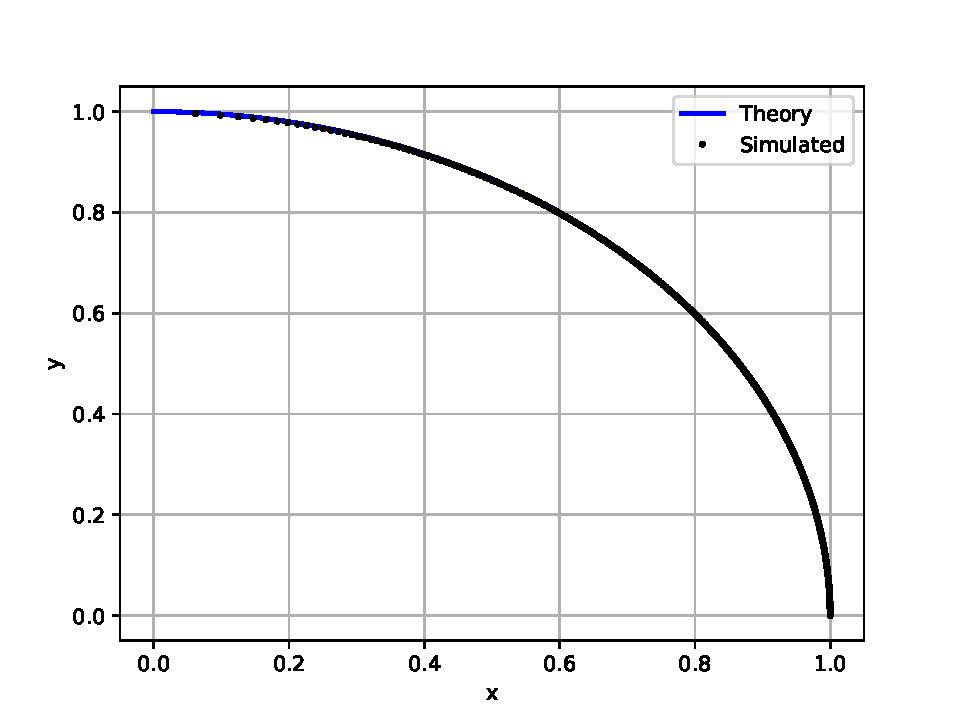
\includegraphics[width=\columnwidth]{figs/fig.pdf}
	\caption{Solution of given DE}
	\label{fig}
\end{figure}

\end{document}
